\RequirePackage{luatex85,shellesc}
\documentclass[crop,tikz,varwidth=4cm]{standalone}
\usepackage{pgfplots}
\usepackage{tikz}
\usetikzlibrary{calc,positioning}
\usepackage{eulervm}
\renewcommand\familydefault{\sfdefault}

\begin{document}

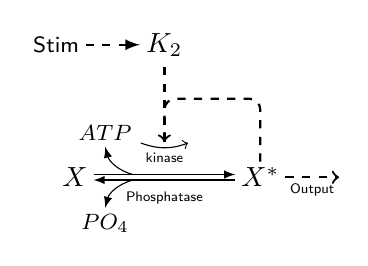
\begin{tikzpicture}[scale=1 , every node/.style={inner sep=2pt} ]

    \node (k1) {$X$};
    \node[right=18mm of k1] (k1p) {$X^*$};

    \edef\o{1}
    \draw[-latex] ([yshift=\o pt]k1.east) -- ([yshift=\o pt]k1p.west) 
        node[midway, label={above:\tiny kinase}] (kinase) {};

    \draw[-latex] ([yshift=-\o pt]k1p.west) -- ([yshift=-\o pt]k1.east)
        node[midway, label={below:\tiny Phosphatase}] (phosp) {};

    % Release P
    \draw[-latex] ($(phosp)+(-0.4,0)$) to[bend right] ++(-135:5mm)
        node[below] {\footnotesize $PO_4$};

    % Consume ATP
    \draw[-latex] ($(kinase)+(-0.4,0)$) to[bend left] ++(135:5mm)
        node[above] {\footnotesize $ATP$};

    % arrow above kinase.
    \draw[->] ($(kinase)+(-0.3,0.4)$) to[out=-20,in=200] node (kinArrow) {} ($(kinase)+(0.3,0.4)$);

    % Kinase autophosphorylate itself.
    \draw[->, dashed, rounded corners, thick] (k1p.north) -- ++(0,0.8) 
        -| (kinArrow.north) node (joina) {} ;

    \draw[-, dashed, thick ] (kinArrow.north) -- ++(0,1) node[above] (k2) {$K_2$};
    \draw[latex-, dashed, thick] (k2) -- ++(-1,0) node[left] {\footnotesize Stim};

    % Neuronal function.
    \draw[->, dashed, thick] (k1p) -- ++(1,0) 
        node[below, midway ] {\tiny {Output} };
    
\end{tikzpicture}	

\end{document}

